\cleardoublepage
\chapter{Introducción y Motivación}
\label{sec:intro} % etiqueta para poder referenciar luego en el texto con ~\ref{sec:intro}
\pagenumbering{arabic} % para empezar la numeración de página con números

Contexto en el que se enmarca el proyecto y la justificación del mismo. Este capítulo es muy importante porque permite al lector conocer qué sentido tiene el proyecto, qué ofrece, por qué es relevante su implementación, los objetivos que persigue, etc. Este capítulo debería tener una extensión de entre 4 y 8 páginas.

\section{Mercado actual de las aplicaciones móviles}

Las aplicaciones móviles han transformado por completo nuestra vida cotidiana. En la actualidad están presentes en nuestra vida diaria y tienen un gran impacto en cómo nos comunicamos, cómo trabajamos, cómo nos divertimos y cómo realizamos nuestras tareas como la compra.

Según los datos de 42matters, compañía que se encarga de recopilar y ofrecer datos a diferentes empresas, el 27 de enero de 2024 hay 2 millones aplicaciones Android en Google Play y algo más de 1.900.000 aplicaciones iOS en App Store, figura~\ref{fig:apps_free_vs_pay}. De las cuales, el porcentaje de aplicaciones que los usuarios se pueden descargar de manera gratuita es aproximadamente de 95\% en ambas tiendas de aplicaciones.

\begin{figure}[H]
\centering
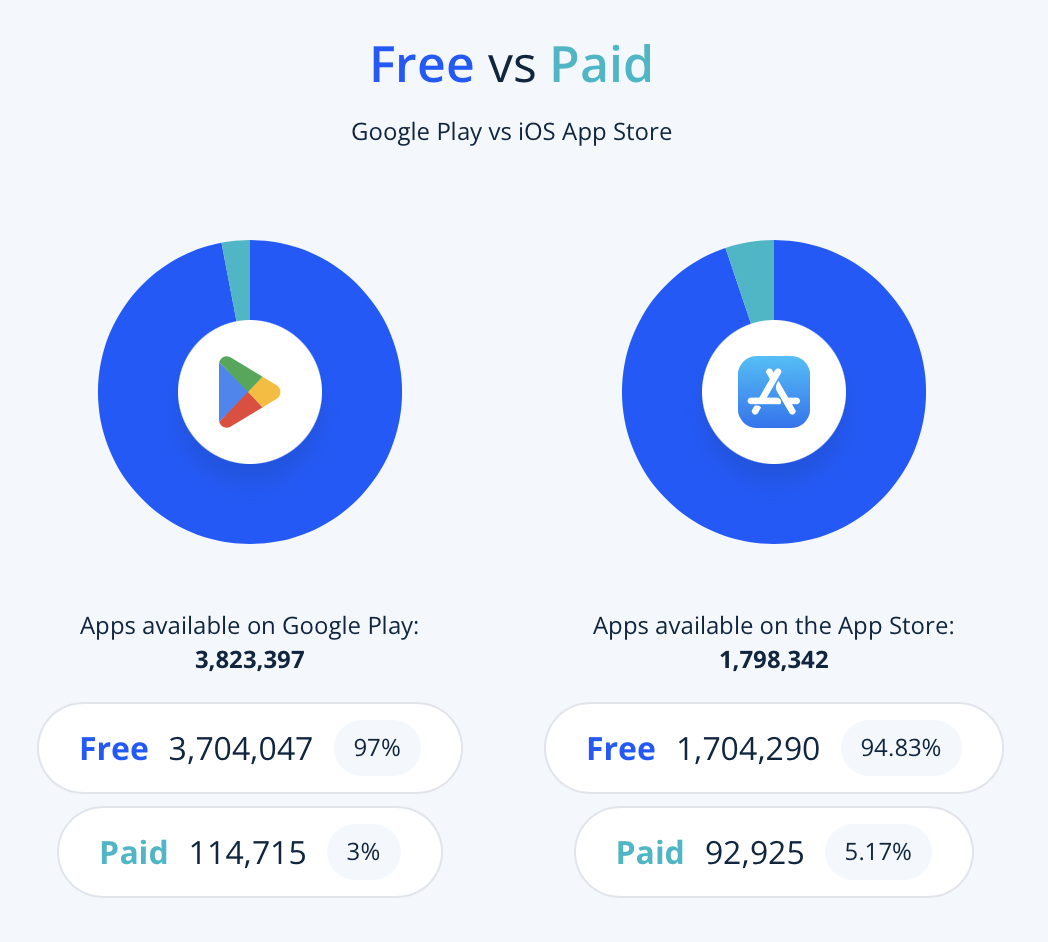
\includegraphics[width=0.6\textwidth]{./img/intro/apps_free_vs_pay.png}
\caption{Aplicaciones gratuitas y de pago, Android vs iOS.}
\label{fig:apps_free_vs_pay}
\vspace{0.2em}
{\footnotesize \centering \textit{Fuente:} \url{https://42matters.com/stats#available-apps-count} \par}
\end{figure}

En cuanto a categorías, figura~\ref{fig:google_play} y figura~\ref{fig:app_store}, la educación lidera en Google Play, mientras que los juegos son predominantes en App Store, apareciendo el “negocio” como segunda categoría en ambos casos.

\begin{figure}[H]
\centering
\begin{minipage}[t]{0.48\textwidth}
\centering
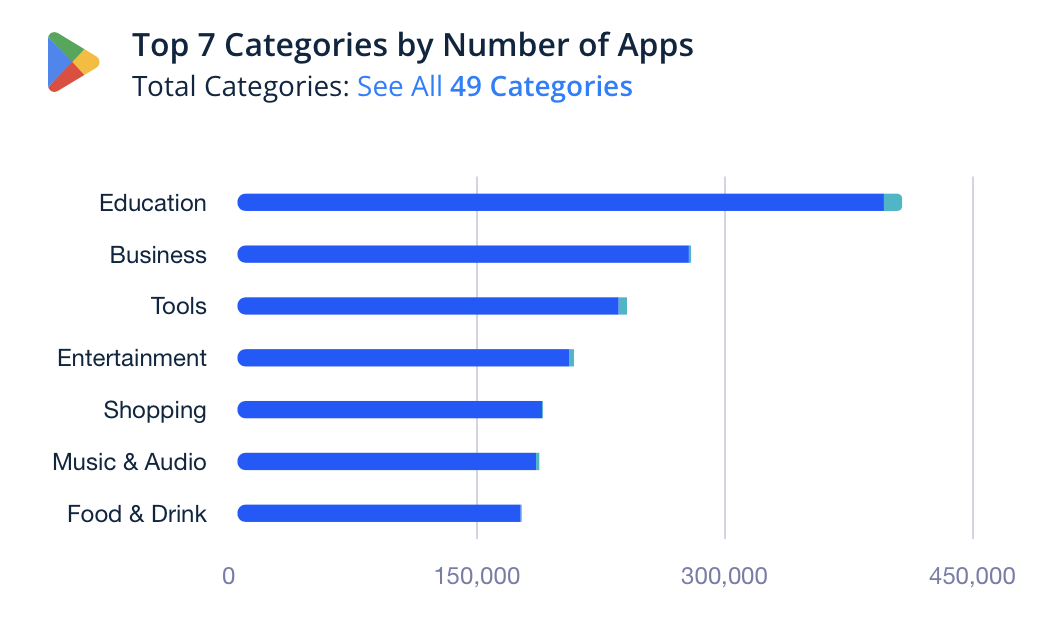
\includegraphics[width=\linewidth]{img/intro/google_play_categories.png}
\caption{Apps por categoría Google Play}
\label{fig:google_play}
\end{minipage}
\hfill
\begin{minipage}[t]{0.48\textwidth}
\centering
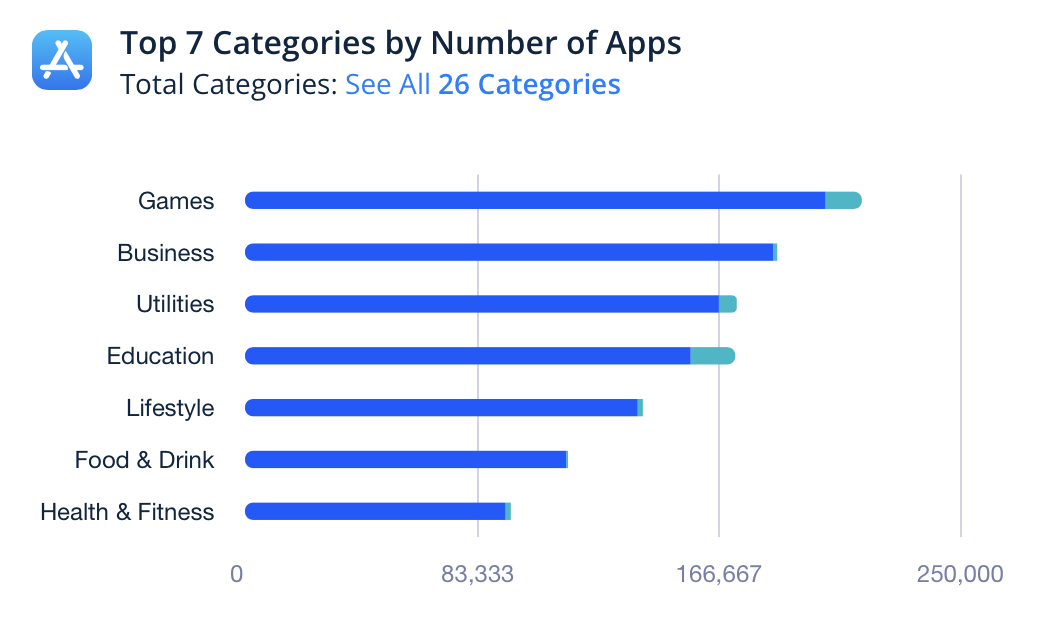
\includegraphics[width=\linewidth]{img/intro/app_store_categories.png}
\caption{Apps por categoría App Store}
\label{fig:app_store}
\end{minipage}
\vspace{0.5em}
\vspace{0.5em}
{\footnotesize \centering \textit{Fuente:} \url{https://42matters.com/stats#apps-by-category} \par}
\end{figure}

Además, se lanzan diariamente más de 2.300 nuevas aplicaciones en Google Play y unas 1.100 en App Store. Esto representa más de 90.000 aplicaciones nuevas al mes en la plataforma de Android, lo que pone de manifiesto la alta competencia y dinamismo de este mercado, figura~\ref{fig:apps_per_month}.

\begin{figure}[H]
\centering
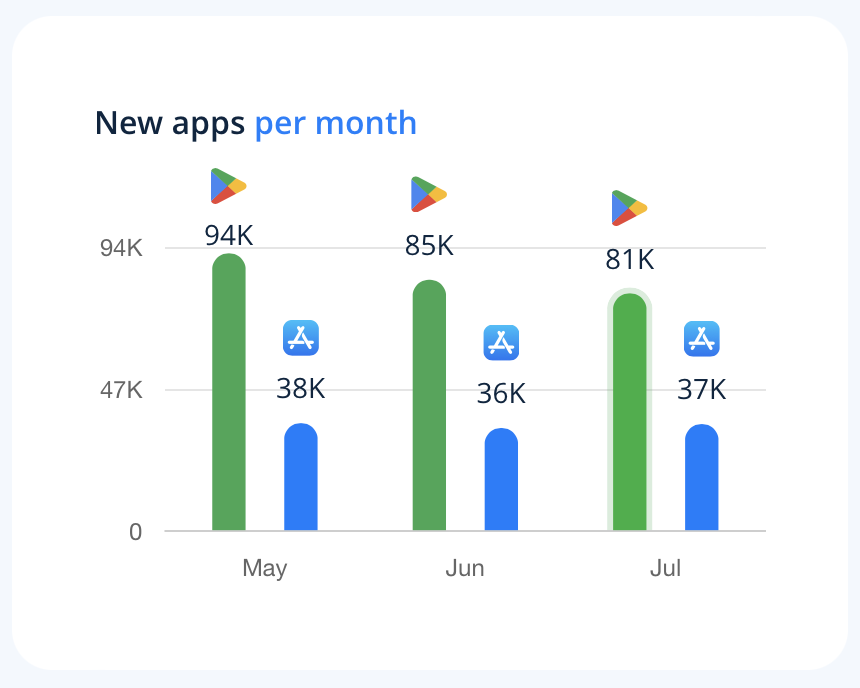
\includegraphics[width=0.7\textwidth]{./img/intro/apps_per_month.png}
\caption{Nuevas aplicaciones por mes en cada tienda de aplicaciones (27/01/2024)}
\label{fig:apps_per_month}
\vspace{0.2em}
{\footnotesize \centering \textit{Fuente:} \url{https://42matters.com/stats#apps-by-category} \par}
\end{figure}

En cuanto a los usuarios, como se puede ver en la figura~\ref{fig:world_map_ios_android}, Android domina el panorama global. Según Statista (junio de 2024), su cuota de mercado alcanza el 72,15\%, frente al 27,19\% de iOS. Aunque en países como Estados Unidos e Irlanda iOS tiene más presencia, en regiones como América Latina, África, Asia y, especialmente, España, Android es el sistema operativo predominante.

\begin{figure}[H]
\centering
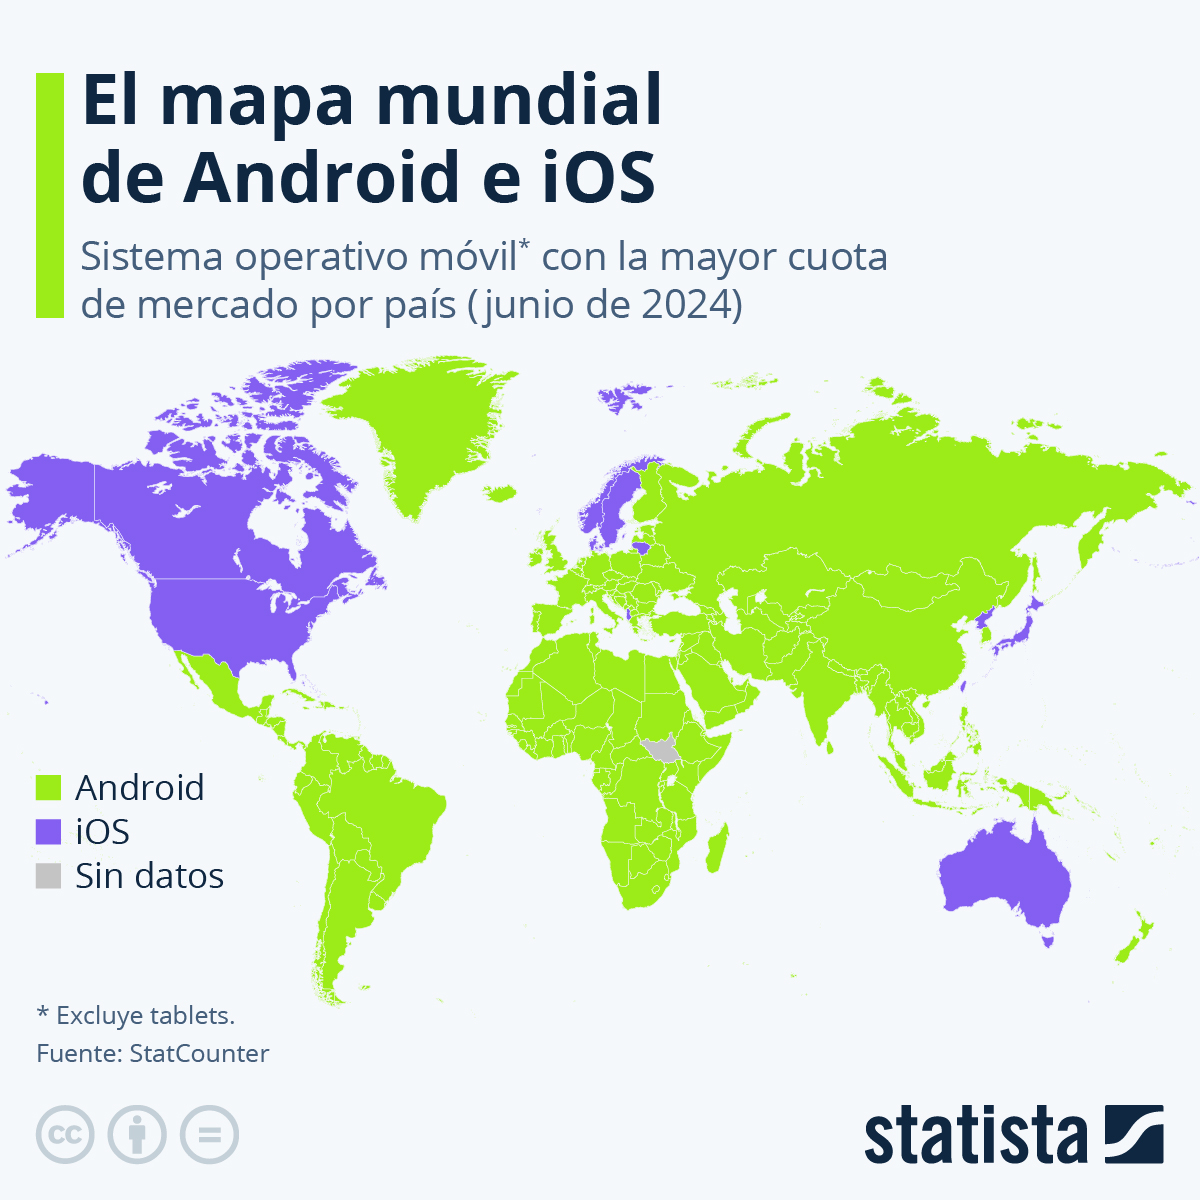
\includegraphics[width=0.7\textwidth]{./img/intro/world_map_ios_android.jpeg}
\caption{Mapa mundial de Android e iOS (27/01/2024)}
\label{fig:world_map_ios_android}
\vspace{0.2em}
{\footnotesize \centering \textit{Fuente:} \url{https://www.statista.com} \par}
\end{figure}

En el caso concreto de España, que es donde se publicaría esta aplicación, el 77\% de los smartphones son Android frente a un 23\% de iOS (Statista, diciembre 2023). Este dato resulta decisivo a la hora de seleccionar la plataforma de desarrollo, ya que permite orientar el producto a la mayoría de los usuarios potenciales.

\section{Tipos de aplicaciones móviles}

El desarrollo de software para dispositivos móviles puede abordarse desde diferentes enfoques según el tipo de aplicación que se desea construir. En general, se distinguen tres tipos principales: aplicaciones nativas, aplicaciones web y aplicaciones híbridas.

Una aplicación nativa es aquella que se crea específicamente para un sistema operativo móvil, utilizando su lenguaje y herramientas oficiales. Esto permite aprovechar al máximo las capacidades del hardware del dispositivo, lo que se traduce en un mayor rendimiento y una experiencia de usuario más fluida. Por ejemplo, una aplicación desarrollada en Kotlin para Android o en Swift para iOS es considerada nativa. Este tipo de desarrollo requiere distribuir la app a través de plataformas oficiales como Google Play o App Store y, en caso de querer abarcar varios sistemas operativos, implica desarrollar una versión distinta para cada uno.

Las aplicaciones web, por el contrario, son páginas web optimizadas para dispositivos móviles, a las que se accede desde el navegador sin necesidad de instalación. Se desarrollan con tecnologías como HTML, CSS y JavaScript, y su principal ventaja es la portabilidad entre sistemas. Sin embargo, su rendimiento es inferior al de una aplicación nativa y tienen acceso limitado a las funcionalidades del dispositivo.

Las aplicaciones híbridas combinan elementos de ambas. Básicamente, se trata de aplicaciones web que se ejecutan dentro de un contenedor nativo, lo que permite distribuirlas desde tiendas oficiales y acceder a algunas funcionalidades del hardware. No obstante, la integración entre la parte web y la parte nativa puede generar complejidades, sobre todo en términos de rendimiento y mantenimiento.

Tras analizar las características de cada enfoque, se optó por desarrollar una aplicación nativa para Android. Esta decisión responde tanto al interés por aprender en profundidad el desarrollo específico para esta plataforma, como al deseo de ofrecer una experiencia más fluida, potente y adaptada a los dispositivos que predominan en el mercado español.

\section{Análisis del entorno}

Antes de iniciar el desarrollo de la aplicación, se llevó a cabo un análisis del entorno para identificar qué soluciones digitales existen actualmente orientadas a la organización de la compra doméstica. Esta revisión permitió detectar tanto buenas prácticas como carencias que justifican el presente proyecto.

Una de las aplicaciones más conocidas en este ámbito es \textit{Bring!}. Su funcionamiento se basa en la creación de listas de la compra mediante una interfaz visual con iconos organizados por categorías (por ejemplo, frutas, lácteos, panadería). Es intuitiva y estética, lo que la hace accesible para usuarios de cualquier perfil. Sin embargo, no permite especificar cantidades con precisión, no admite comentarios o notas personalizadas para cada producto, ni se integra con recetas o planificación semanal, lo que limita su utilidad para quienes desean gestionar la compra de forma más detallada.

Otra opción popular es \textit{Listonic}, que apuesta por un diseño más clásico: listas de verificación con productos agrupados por secciones del supermercado. Es rápida y práctica, y ofrece sugerencias inteligentes basadas en el texto introducido por el usuario. No obstante, su interfaz resulta más básica y no incorpora funcionalidades como la planificación de menús, el control del consumo habitual o la personalización de listas según hábitos domésticos.

Ambas aplicaciones ofrecen soluciones útiles para el usuario promedio, pero presentan limitaciones cuando se busca una herramienta más flexible y adaptada a la realidad diaria de una persona o familia que necesita controlar mejor lo que compra, cuándo lo compra y por qué. Esta falta de personalización y de conexión con hábitos reales de consumo doméstico justifica el desarrollo de una alternativa más completa y adaptable.

A diferencia de otras soluciones del mercado, Pinche aborda el problema de la organización de la compra doméstica desde una perspectiva práctica, personalizada y centrada en la realidad cotidiana de quienes gestionan los menús y las compras del hogar.

La aplicación se estructura en tres secciones funcionales: listas de la compra, recetas e invitados. En la sección de listas, el usuario puede crear múltiples listas adaptadas a distintas ocasiones —por ejemplo, “Lista semanal” o “Cumpleaños de María”— y añadir productos con su cantidad, e incluso el supermercado donde se prefiere comprarlos. En la sección de recetas, se pueden almacenar platos con su elaboración detallada e ingredientes para un número determinado de comensales, además de añadir fácilmente esos ingredientes a cualquier lista activa. Por último, en la sección de invitados, se puede registrar información personalizada sobre las personas que suelen comer en casa, como sus intolerancias, preferencias y qué platos se les han preparado recientemente.

Esta estructura modular convierte a Pinche no solo en una herramienta para digitalizar listas de la compra, sino en una solución doméstica integral que facilita la planificación, optimiza el tiempo y mejora la experiencia culinaria y organizativa en el hogar. Al permitir registrar hábitos, preferencias e información nutricional, contribuye también a evitar errores comunes como compras duplicadas, olvidos o preparación de menús inadecuados para los invitados.

Desde el punto de vista académico, el proyecto ofrece un caso completo para aplicar competencias clave del grado: desarrollo de interfaces modernas con Jetpack Compose, gestión de datos con Firebase, diseño orientado al usuario y trabajo bajo metodologías ágiles.

En definitiva, Pinche es un proyecto que trasciende el ejercicio académico. Es una propuesta aplicable y escalable, que puede mejorar la calidad de vida de los usuarios al resolver un problema doméstico frecuente mediante una herramienta accesible, inteligente y bien estructurada.